\chapter{Conclusion}
\label{chap: Chapter 8}

Based on the discussion in the previous chapter, it is clear that using various Natural Language Processing and text mining techniques outlined in chapter \ref{chap: Chapter 6} would indeed be possible.
It was apparent that adjusting the parameters of the prototype also played a major part in the quality of the topics. Later such topics directly influenced the recommendation list.

This chapter provides a summary of the study to conclude the study findings. The next section will discuss how the research objectives were reached. After the section of how the research objectives were accomplished, suggestions for future research will be made.

\section{Revisiting the research objectives}

This section facilitates a discussion on how the research objectives were met. As mentioned in chapter 1, the primary research objective was to \textbf{\textit{Develop a model to recommend related research papers.}}

Achieving the primary objective depended on meeting the secondary objectives listed in Chapter \ref{chap: Chapter 1}.

\textbf{SO 1}: \textit{To identify recommender systems techniques and how they are used.}

This secondary objective was met by surveying the literature of Recommender Systems. As this secondary objective's goal was to map and understand what techniques are used in recommender systems and how researchers utilise it. I looked at the various approaches that not only fits the use case of the study but also which is relevant. It was decided that the Content Based Filtering approach would the best to use since no assumptions are made of users activity. In addition to this, CBF does not care about user ratings, it looks at the content of the documents. It was critical to look for approaches that does not rely on user activity and user ratings. Chapter \ref{chap: Chapter 2} was dedicated to introduce the concepts of how modern Information Systems (Recommender Systems) work and how they evolved from the past to recent years. A continuation on the introduction to the fields was found in Chapter \ref{chap: Chapter 3}.

\textbf{SO 2}: \textit{To identify machine learning techniques that assist with the recommender task.}

This secondary objective was met by surveying several machine learning techniques. The goal of this objective was to identify and better understand what machine learning techniques there are, and how they tie into recommender type systems.
Machine Learning in section \ref{ssec:MLoverview}, Natural Language Processing in section \ref{secc:LDAover} and Topic Modeling in section \ref{ssec:tmodel} paved the way to understand the technology that would be used in this study.

The selection of the topic model algorithm that would be most suitable came from literature. More specifically in section \ref{ssec:tmodel} it was discussed that Latent Dirichlet Allocation (LDA) was a very popular choice for building such topic models. Furthermore, section \ref{ssec:LDAA} explains how LDA works, by computing hidden topic structures from documents.

The main research objective was met by consolidating \textbf{SO 1} and \textbf{SO 2} to form a conceptual model. The model was refined by developing a prototype. While developing the prototype components outlined in the conceptual model Chapter \ref{chap: Chapter 5} were used. 

To develop such a model some guidance were needed. The researcher used the data analytics lifecycle process to harness work done by secondary objective one and two.
Further refinement was needed on the model to display research rigor. 

A prototype was developed to refine, ensure amendments to be done and evaluate the model. The development of the model was documented in Chapter \ref{chap: Chapter 5} and accompanied by the development of the prototype in Chapter \ref{chap: Chapter 6}. Using the prototype the model was evaluated to show if it is applicable and feasible. Furthermore, the model demonstrated applicability since it requires domain specific data for training and it was done using information security South Africa conference data.
In addition to that, the model also demonstrated feasibility with the ease of using recommender system and machine learning techniques.

In the next section, a reflection of the model will be discussed.

\section{Reflection on the Model}

\begin{figure}[htbp]
\centering
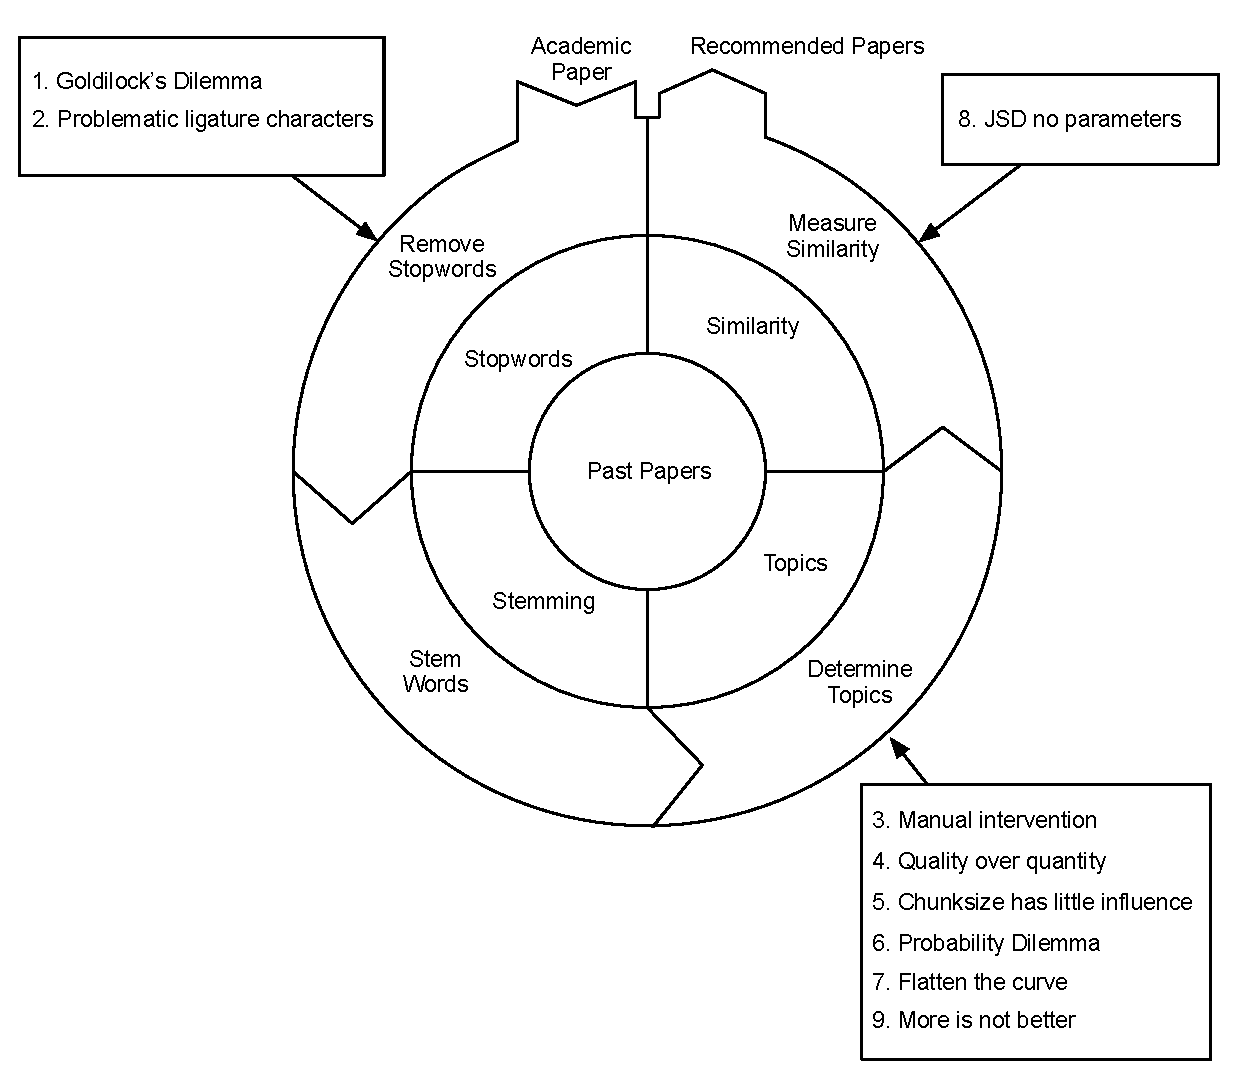
\includegraphics[width=15cm]{./figures/Lesson77.eps}
\caption{Mapping lessons learned to the model}
\label{fig:processing1}
\end{figure}

This section reflects on the model and the accompanying prototype. The model was set out to identify related research papers. The model specified the process that needs to be followed and the prototype showed that it is indeed feasible to implement. The prototype showed that it worked within the specific domain of information security papers since we used information security South Africa conference papers from 2006 - 2016 as data. Addressing the main objective using the model and prototype, I showed that it can be done theoretically and practically.

The prototype served a dual purpose. The first is to learn technologies and gain first hand experience related to recommender systems. The second was to demonstrate the applicability by using various technologies and feasibility by using a information security specific domain. 

The majority of the lessons learned exists on the topics quadrant of the model as depicted in Figure \ref{fig:processing1}. I found that removing the stopwords and stemming the data has been streamlined and the body of knowledge is well defined. Removing stopwords and stemming presents two lessons to draw future researchers attention to the subtleties in the area. For testing similarity measures only Jensen-Shannon Divergence was tested. Jensen-Shannon Divergence does not use parameters, and therefore had an big influence on the preceding steps.
This opens up opportunities for future research to be done using different similarity measure technologies which contains parameters. 

To get back to the majority of the lessons about determining the topics. Lessons four, seven and nine shows us that if we can better define the domain the model will perform better. A trade-off between accuracy and generality thus exist. In the prototype the domain was limited to information security papers by using research papers from the information security South Africa conference. 

Moving on to lesson three, manual intervention. I found that evaluation techniques for machine learning algorithms are well defined and streamlined. However, human validation are still needed as bad topics still make it into the system. Thus challenging further researchers to look for methods and techniques that eliminates such human intervention altogether. 

\section{Research Limitations}
This study has some limitations that must be recognized. The first limitation is that of the sample size. At the time of data collection, the information security South Africa conference only had 254 research papers to use in the dataset. Of that 254 research papers certain topics are discussed in a small number. If the topics are scarce during training, the recommendation task will be very difficult to complete. The goal was to train and test the prototype using one specific library of one conference.

The second limitation is that only one topic modeling technique (Latent Dirichlet Allocation) was used. There were several reasons behind it namely, recent research suggested that when using Content-based approaches, Latent Dirichlet Allocation would be preferred. 
Considering time constraints as this is a Masters study, we felt to go ahead with the one topic modeling technique.

The third limitation, this study only uses Jensen-Shannon Divergence to calculate the similarity between the two data spaces (Test set and training set). Similar to the second limitation, time did not allow us to venture deeper into different similarity measures.

Lastly, the forth limitation includes not having a human factor to evaluate each phase individually. The phases which are referred to is the outputs of the Topic Modeling technique and, also the end result of the similarity measurement. 

\section{Suggestions for further research}
This section is dedicated to outline further research to be done on the limitations which was raised in the previous section. Future research could possibly be conducted using a conference that has more research papers to their disposal. It will provide more data to be clustered and ultimately better the similarity measures. This relates to the first limitation.

Reflecting on the second limitation, the study could include multiple Topics Modeling algorithms and compare the outputs. Algorithms like Non Negative Matrix Factorization (NMF) \cite{Purpura2018}, Latent Semantic Analysis (LSA) \cite{Qomariyah2019}, Parallel Latent Dirichlet Allocation (PLDA) \cite{Mukherjee2019} and Pachinko Allocation Model (PAM) \cite{Koltcov2021}. 

Similarly, the third limitation, using different similarity measures could lead to different recommendations. Furthermore, mixing different Topic Models with similarity measures could yield better results.

The forth limitation which includes human intervention to evaluate each phase could speed up the model implementation, since getting feedback every step of the way. Suggestion for further research can include looking for methods and techniques that eliminates manual intervention.

\section{Epilogue}
This study identified that it's time consuming for researchers to look for related research papers. This problem was addressed by developing a model to recommend related research papers. During the development of the model and prototype, it was evident that machine learning bridges the gap of spotting latent themes. However, the lessons learned Chapter \ref{chap: Chapter 7}, shows that when other researchers endeavour onto similar topics a great learning curve awaits. The researcher hopes that this study motivates other researchers to advance the natural language processing and machine learning research angle traditional topics.

